\documentclass[tikz,border=5pt]{standalone}
\usepackage{amsmath,amssymb,fontspec,unicode-math}
\setmainfont{STIXTwoText-Regular.otf}
\setmathfont{STIXTwoMath-Regular.otf}
\usetikzlibrary{positioning,arrows.meta,calc,decorations.pathreplacing}
\definecolor{hmtgray}{gray}{0.3}
\definecolor{hmtblue}{gray}{0.15}
\definecolor{hmtgold}{gray}{0.3}
\definecolor{hmtgreen}{gray}{0.1}
\definecolor{hmtred}{gray}{0.25}
\definecolor{hmtlightblue}{gray}{0.92}
\definecolor{hmtlightgold}{gray}{0.83}
\definecolor{hmtlightgreen}{gray}{0.97}
\definecolor{hmtlightred}{gray}{0.73}
\begin{document}
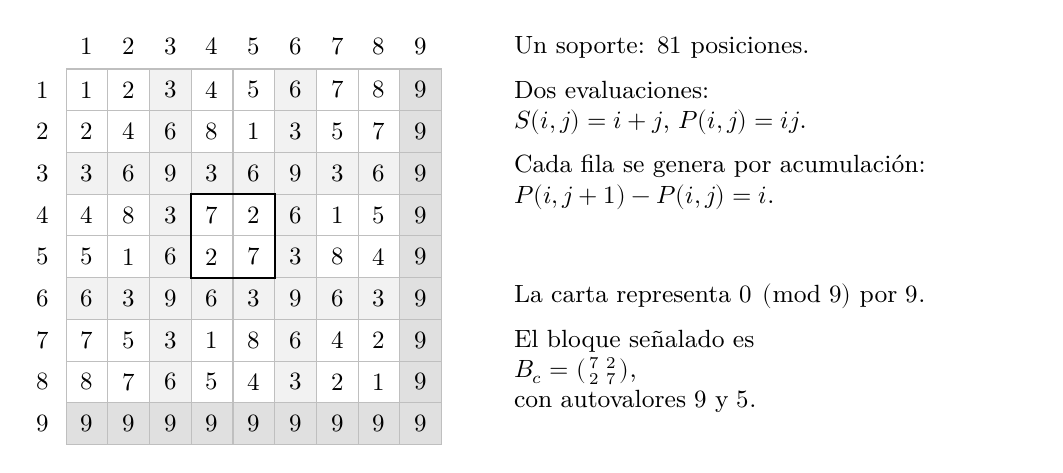
\begin{tikzpicture}[x=.53cm,y=.53cm,font=\small]
\fill[black!5] (1.5,-.5) rectangle (2.5,8.5);
\fill[black!5] (4.5,-.5) rectangle (5.5,8.5);
\fill[black!5] (-.5,2.5) rectangle (8.5,3.5);
\fill[black!5] (-.5,5.5) rectangle (8.5,6.5);
\fill[black!12] (7.5,-.5) rectangle (8.5,8.5);
\fill[black!12] (-.5,-.5) rectangle (8.5,.5);
\foreach \i in {1,...,9}{
 \node at (\i-1,9.05) {\(\i\)};
 \node at (-1.05,9-\i) {\(\i\)};
 \foreach \j in {1,...,9}{
  \pgfmathtruncatemacro{\v}{mod(\i*\j-1,9)+1}
  \node at (\j-1,9-\i) {\(\v\)};
 }
}
\foreach \k in {0,...,9}{
 \draw[black!25] (\k-.5,-.5)--(\k-.5,8.5);
 \draw[black!25] (-.5,\k-.5)--(8.5,\k-.5);
}
\draw[line width=.65pt] (2.5,3.5) rectangle (4.5,5.5);
\node[anchor=west,align=left,text width=6.5cm] at (10,7.2) {Un soporte: \(81\) posiciones.\\[5pt]Dos evaluaciones:\\ \(S(i,j)=i+j\), \(P(i,j)=ij\).\\[5pt]Cada fila se genera por acumulación:\\ \(P(i,j+1)-P(i,j)=i\).};
\node[anchor=west,align=left,text width=6.5cm] at (10,1.8) {La carta representa \(0\pmod9\) por \(9\).\\[5pt]El bloque señalado es\\ \(B_c=\left(\begin{smallmatrix}7&2\\2&7\end{smallmatrix}\right)\),\\ con autovalores \(9\) y \(5\).};
\end{tikzpicture}
\end{document}

